%04chapterSelbsteinsch.tex
\chapter{Selbsteinschätzungen}
In diesem Kapitel wird beschrieben, welche Rollen die Teammitglieder mittels Selbsteinsch"atzung erhalten. Dazu wird ein Test verwendet, welcher urspr"unglich von R.M. Belbin \cite{belbin1981management} entwickelt und an der Universit"at Regensburg ins Deutsche übersetzt wurde. In diesem Test werden verschiedenste Aussagen bezüglich des eigenen Verhaltens in bestimmten Situationen mittels eines Punktesystems bewertet. Am Ende trägt man die Punkte in ein Raster ein, aus welchem sich dann die passenden Rollen herauskristallisieren.

\subsection*{Pascal Horat}
Da ich in meinem Leben schon andere, ähnliche Tests ausgefüllt habe, wusste ich welche Rollen ich als Resultat in etwa zu erwarten hatte. Trotzdem war ich gespannt, ob sich auch dieses Mal dieselben Tendenzen zeigen würden. \\

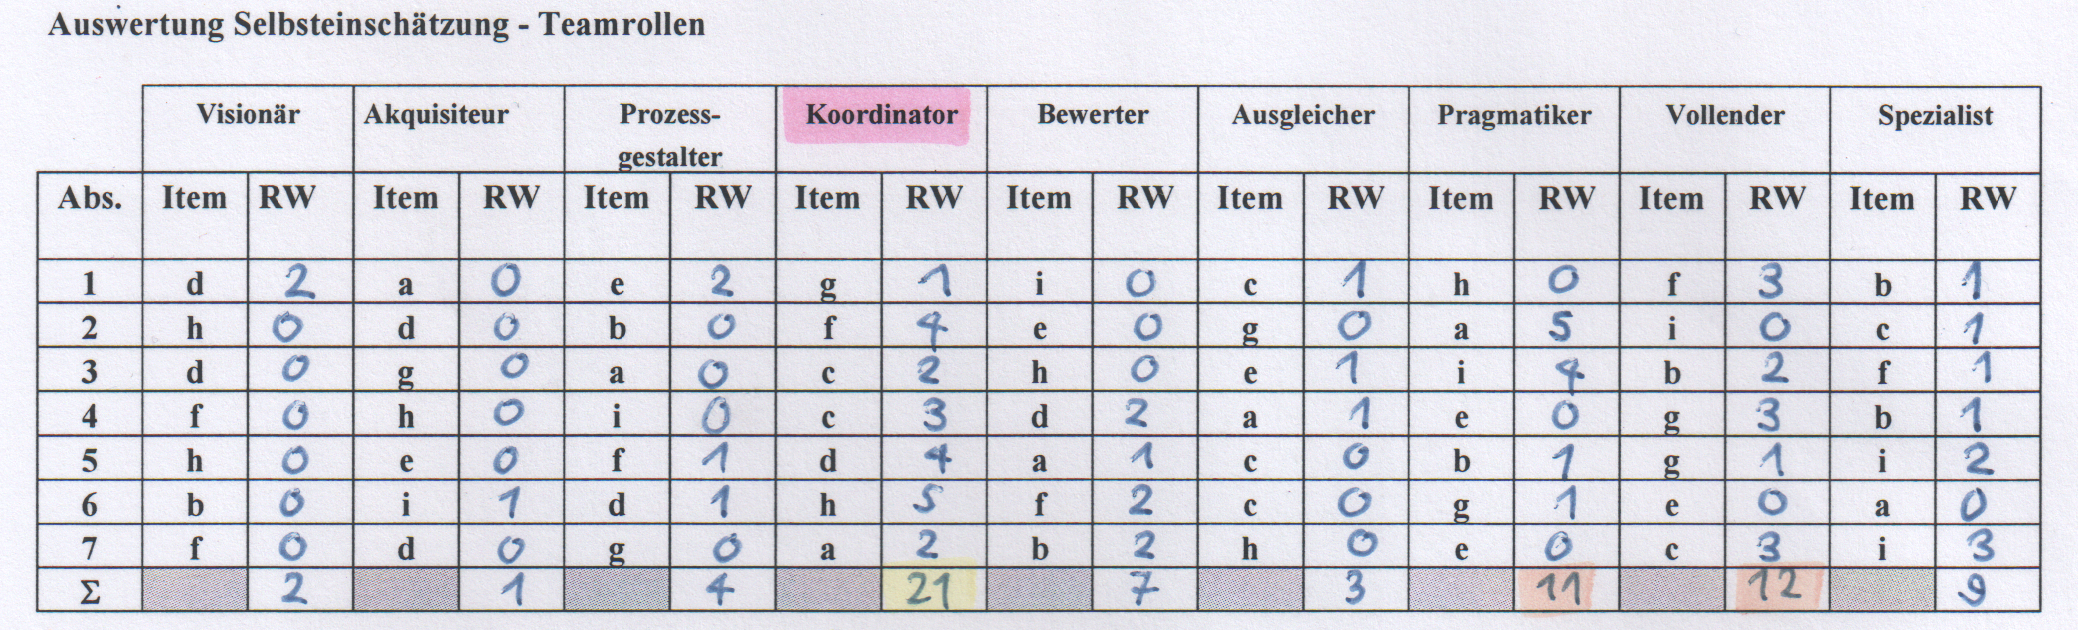
\includegraphics[height=39mm]{images/SelbsteinschaetzungHorat.png}

Tatsächlich erreichte, wie von mir im vornherein erwartet, die Rolle des Koordinators die höchste Punktzahl. Allerdings war ich überrascht mit welcher Deutlichkeit das Resultat ausfiel. Wie in obiger Grafik ersichtlich, haben die Rolle des Pragmatikers und des Vollenders die zweitgrösste Ausprägung (orange markiert). Auch sieht man, das die Visionärsrolle und die des Akquisiteurs fast keine Punkte erhalten haben. Die äusserst niedrige Punkteausbeute beim Visionär hat mich eher überrascht. Ich finde nämlich, das oft alternative Ansätze und neue Ideen von meiner Seite kommen.

\subsection*{Steve Gerome Kamga}
Das Resultat meiner Auswertung mit der Belbin-Methode hat einige Teamrollen aufgezeigt, die zu meinen Fähigkeiten und meinem Verhalten bezüglich der Zusammenarbeit passen könnten. Nachfolgend werden die drei Teamrollen erwähnt, bei denen ich die meisten Punkte bekommen habe.
Als erstes kommt der Pragmatiker, der sich als eine auf die anstehende Sache und entsprechendes praktisches Handeln gerichtete Person definieren lässt. Danach folgen der Spezialist und der Vollender.
\newline
Nach dieser Bewertungsmethode habe ich in Ruhe die drei obengenannten Teamrollen überdacht und mir einige persönlichen Fragen gestellt. Resultierend würde ich sagen, dass die Ergebnisse bei mir mindestens zu 60\% stimmen, obwohl die Belbin-Methode nur auf Einschätzungen basiert.


\subsection*{Gökhan Kaya}

Meine Auswertung der Selbsteinschätzung gemäss Belbin ergab die folgende Punkteverteilung:

\begin{tabular}{lr}
  Visionär & 2 \\ 
  Akquisiteur & 5 \\ 
  Prozessgestalter & 8 \\ 
  Koordinator & 10 \\ 
  Bewerter & 2 \\
  Ausgleicher & 19 \\
  Pragmatiker & 7 \\
  Vollender & 6 \\
  Spezialist & 11 \\
\end{tabular}
\newline


Somit ist zu sehen, dass folgende drei Teamrollen herausstechen:
%\renewcommand{\labelenumi}{\roman{enumi}} 
\begin{enumerate} 
\item Ausgleicher 
\item Spezialist
\item Koordinator
\end{enumerate}

Wobei besonders die Rolle des Ausgleichers mit 19 Punkten hervorsticht. Dies war für mich keine Überraschung, da sich während den Teamsitzungen bereits herauskristallisierte, dass der gute Teamzusammenhalt einer meiner Hauptziele geworden war. Ich habe mich entsprechend eingesetzt und immer wieder versucht herauszufinden, ob alle mit den getroffenen Entscheidungen zufrieden waren und wirklich nichts auszusetzen hatten. Falls doch habe ich versucht, mir die Meinung jedes einzelnen anzuhören und auszudiskutieren.

